%!TEX root =  ../main.tex

\objective{Compose and cecompose sums of power functions}

\subsection{Curvilinear Asymptotes}
We said last section that a rational function where the degree of the numerator is greater than
the degree of the denominator will have an asymptote defined by the quotient of the two,
ignoring the remainder.  Let us see an example.

$$
f(x)=\frac{(x+1)(x-2)(x-5)(x+5)}{(x-1)(x+2)}
$$

We can see that the first and last terms of the top will be $x^4 \dots +50$.  The bottom 
multiplies out to$x^2+x-2$.  The first two and the last two pairs in the numerator are easy 
to multiply: $(x^2-x-2)(x^2-25)$.  While a bit tortuous, multiply two trinomials is certainly
the easiest way to find the numerator, and it is $x^4-x^3-27x^2+25x+50$.  We can now find
the curvilinear asymptote.

\polylongdiv{x^4-x^3-27x^2+25x+50}{x^2+x-2}

The asymptote is a parabola!  It opens upward, has a $y$-intercept of -23 and a centerline 
at $x=1$.

\begin{figure}
\begin{centering}
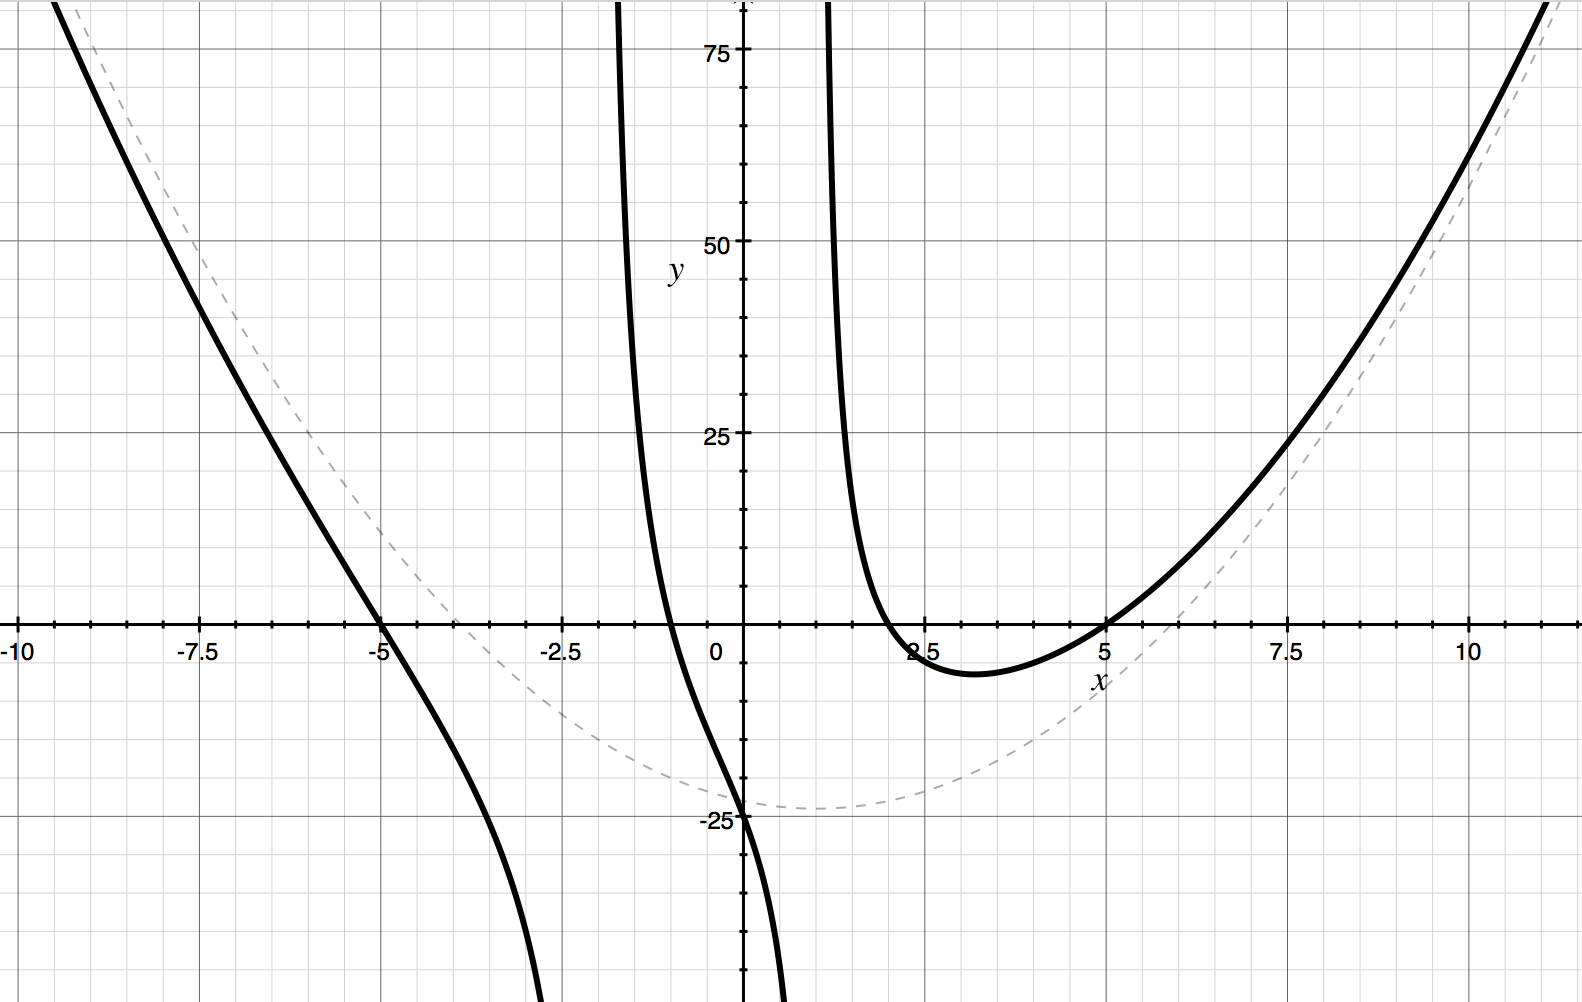
\includegraphics[width=\textwidth]{\chapdir/pics/curvilinear}
\caption{A function with a parabolic asymptote}
\end{centering}
\end{figure}

\subsection{Partial Fraction Decomposition}
Calculus is not concerned what the function does everywhere: we have the function itself
for that.  Calculus is satisfied local behavior, what a function does nearer and near to
certain places.  The curved asymptote we just found is more and more right, the larger 
(positive or negative) a number we plug into it.  We know how to find lines that behave
live the function almost any other point on the graph: tangent lines with a slope from
the derivative.  For example, at (5,0), the behavior can be modeled with 
$y-0 = \frac{47}{5}(x-5)$.  But what about around the asymptotes, at 1 and -2?  That is
where we bring back the ``remainder'' from the polynomial long division.

$\frac{44x+4}{x^2+x-2}$ is the non-asymptote part of the quotient, which we know is 
composed of $(x-1)(x+2)$ in the denominator.  Is there some way to rip it apart, into
two fractions, one with a denominator of (x-1) and another with (x+2)?  Let us suppose
there is, and that each fraction has a simple constant in the numerator.  That would
mean we are hypothesizing

$$
\frac{A}{x-1} + \frac{B}{x+2} = \frac{44x+4}{x^2+x-2}
$$

where $A$ and $B$ are plain numbers.  We can begin to figure out what they are by
``clearing the fraction'', multiplying by $x^2+x-2$ on both sides.  By factoring and canceling,
we get

$$
A(x+2) + B(x-1) = 44x + 4
$$

If we distribute and group for like terms, we get

$$
(A+B)x + (2A-B) = 44x + 4
$$

Now we already said $A$ and $B$ are numbers, so if we have $A+B x$'s on the left,
then $A+B$ must equal 44, and $2A-B$ must equal 4.  We can either add these two 
equations, or use a matrix and find that $A=16$ and $B=28$.  This means $\frac{16}{x-1}
+ \frac{28}{x+2} = \frac{44x+4}{x^2+x-2}$.

Additionally, we have decomposed the fraction into its partial fraction components,
a fancy way of saying we made it easy to integrate.  This assume that you know that
$\int \frac{1}{x} = \ln{|x|}$, which we will not prove until chapter 8.

In the vicinity of $x=1$, $\frac{16}{x-1}$ is a good model, and in the vicinity of $x=-2$,
$\frac{28}{x-2}$ is a good model of $f(x)$.


\subsection{Sums of Power Functions}
Finally, everything we have learned up until this point is also good for sums of 
power function that do not obey the definition of polynomials and rational functions.
For example, suppose you wanted to make a doorway modeled by the equation
$h(x) = \sqrt[3]{(x+4)^2}+\sqrt[3]{(x-4)^2}$ from -4 to 4.  If you had to program a 
machine lathe to make the curved top, what would its slope be at every point
on the interval?

We will need both the integral and the derivative of the function, but fortunately
it is the Power Rule all around.  $h'(x) = \frac{2}{3\sqrt[3]{x+4}}+\frac{2}{3\sqrt[3]{x-4}}$
and $H(x) = \frac{3}{5}\sqrt[3]{(x+4)^5}+\frac{3}{5}\sqrt[3]{(x-4)^5}+C$
